% Experiments chapter.
%
% Developed for my Master Thesis at Maastricht University.
% Based on Eugenio Senes's template at the University of Torino.
%
% By Joeri Hermans (joeri@joerihermans.com)
%
% Released under an MIT license. Share, modify and enjoy, but quote the author!

\chapter{Experiments}
\label{chapter:experiments}

This chapter describes the experiments, and their results, we conducted to obtain emperical evidence for our hypotheses. We start by applying our theories to a well-studied problem such as MNIST~\cite{mnist}. Afterwards we apply our knowledge to CERN specific problems, such as track reconstruction and event identification.

\section{Handwritten Digit Classification}
\label{sec:experiment_mnist}

\section{CMS Track Reconstruction and Event Identification}
\label{sec:experiment_track_reconstruction}

To reduce the computational load of collision reconstructions in future LHC runs, the CMS experiment is exploring Machine Learning techniques as a possible approach for accomplishing this. In this particular case, the experiment is evaluating Deep Learning techniques by fitting them to physics problems, more high-level problems such as deciding which data to keep in the High Level Trigger, and other inference problems. In the following experiments, we mainly occupy ourselves with the reconstruction of \emph{particle tracks}, and identification of \emph{track types} from raw detector \emph{hits}. A particle track, \emph{track} denoted from this point on, is the path that has been traversed by a particle through the detector. The track is reconstructed from a set of hits, which have been triggered (detected) by parts of the detector. The reconstruction of these tracks is a computationally intensive process, since given a set of hits, one needs to minimize the $\chi^2$ error of the track with respect to the set of hits that have been associated with a particular track. However, this is only one aspect of the problem, one first needs to obtain the set of hits which describe a track given all hits within a collision, which also includes the background (false-positives) generated by the detector itself. Currently, the set of hits related to a single track are extracted using a two-pass Kalman filter, with the first pass starting on the outer edges of the detector.\\

An additional problem of applying Deep Learning, or any other Machine Learning approach to the problem of track reconstruction, or event identification, is the petabyte scale data that needs to be dealth with. A simple, and more common solution would be to sample a more managable fraction of the dataset to train our models on. However, we want the model to be able to extract as many diverse tracks as possible that have been reconstructed over previous years by the reconstruction software. As a result, a distributed (data parallel) approach is necessary. However, the data representation is also an important aspect of the problem. Currently, all collisions are stored in the \textsc{root} format, where every reconstructed track for a particular collision (or set of collisions), including the hits of the track, and track parameters can be extracted from. This specific data format is quite problematic, especially taking the petabyte-scale data into account. Furthermore, depending on the modelling, the data needs to be preprocessed in a particular way. One could of course preprocess the complete physics data in a format and shape the models accept, and simply copy the data to the machines which will be used during training. However, this is not a very space efficient approach.\\

A more reasonable, and space efficient approach would be to deliver the preprocessed data to the training procedure in a streaming manner. For example, every worker has a buffer in which it will prefetch and preprocess data coming from the \textsc{root} format in a way the model will understand, e.g., \textsc{numpy} arrays. This approach does not have the space inefficiencies the previous approach had. However, there is an increased computational load on the worker nodes due to the prefetching, and preprocessing of the data. Nevertheless, compared to computation of gradients, this load is neglecktable. An additional benefit of this approach is that the same architecture can be used during model development, since data representations can be generated on-the-fly.\\

\subsection{Data Representation}
\label{sec:experiment_cms_data_representation}

As stated above, our problem can be described as ``\emph{given a set of hits for every collision, identify the (sub)set of hits which belong to a specific track}''. In a first step, we simplified the problem as: \emph{given a set of hits of a collision, identify the types of tracks that occurred in said collision}. Using this simplified version of the problem statement, we could experiment with data representation, and model topology quite easily, without having to think about the modelling of the tracks. Our initial idea was to construct a three-dimensional ``image'' of the detector, where the image is basically a discretized heatmap of the hits in the detector. However, in order to maintain the required resolution in the inner part of the detector, without sacraficing dimensionality of the parameterization of the model, we had to limit the data representation to a two-dimensional approach. In this two-dimensinal approach, we construct two \emph{feature matrices}. One matrix represents the front-side of the detector, along the beam-axis, and the other, perpendicular to the beam-axis, represents the side of the detector. Since every hit is a three-dimensional coordinate, constructing these matrices is quite straightforward.

\begin{figure}[H]
  \centering
  \begin{subfigure}{.48\textwidth}
    \centering
    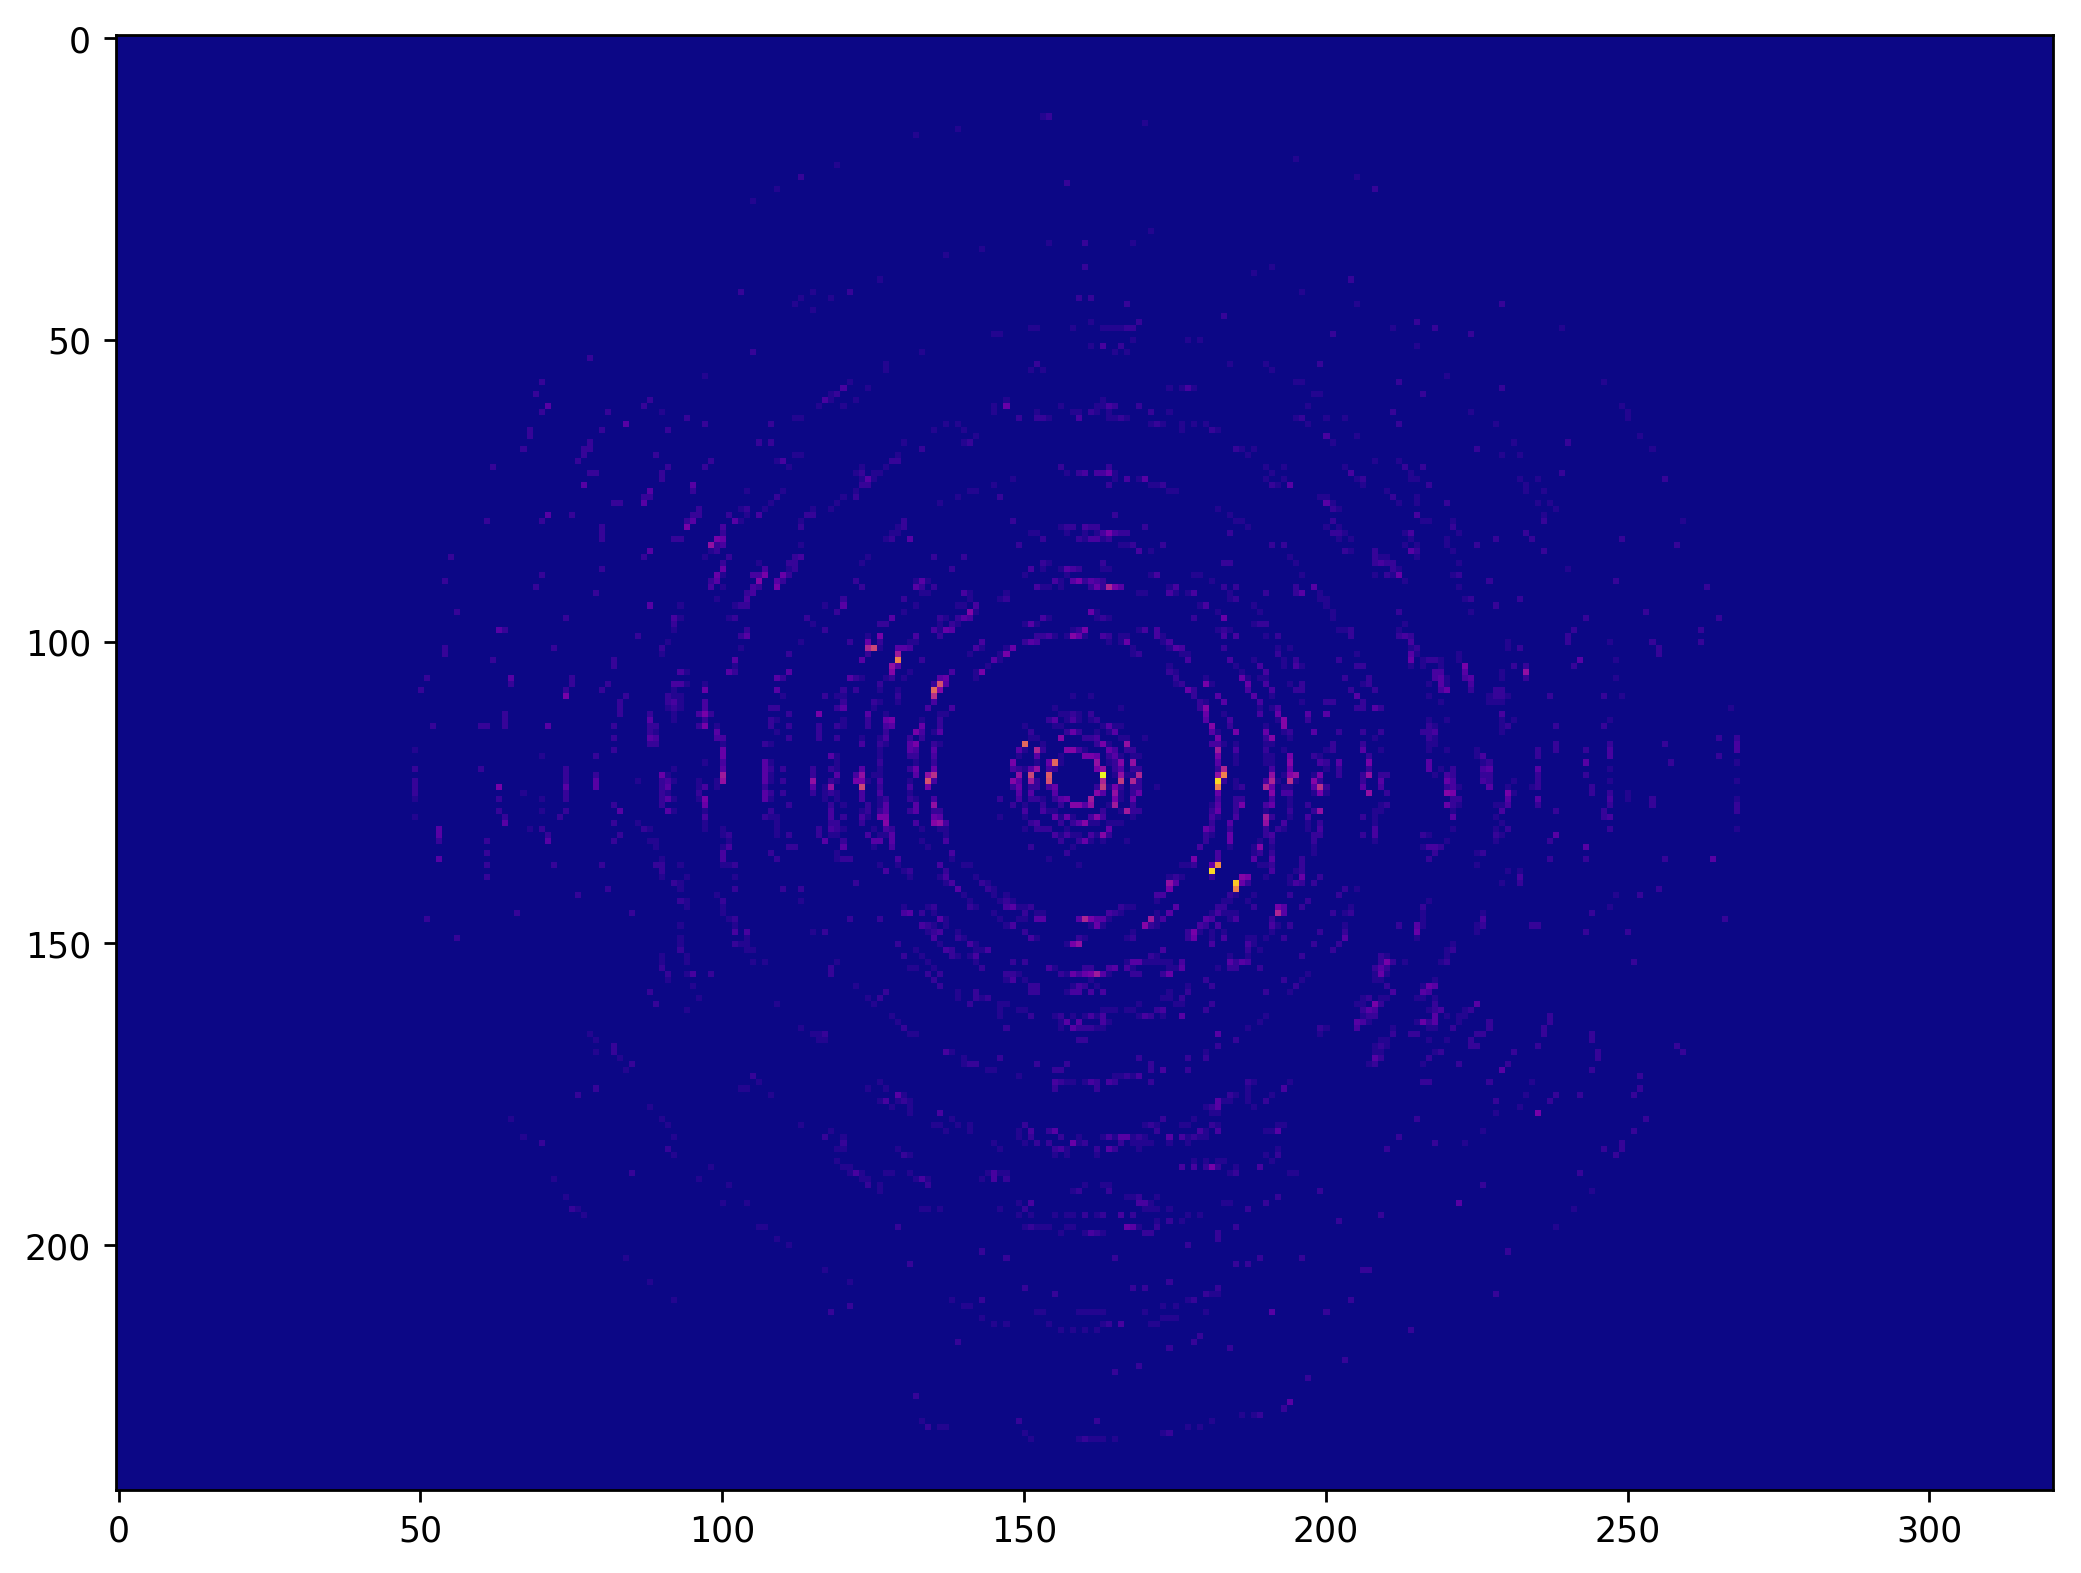
\includegraphics[width=\linewidth]{resources/images/experiment_cms_tracking_1}
    \caption{Subfigure 1}
    \label{fig:experiment_cms_input_1}
  \end{subfigure}
  \begin{subfigure}{.48\textwidth}
    \centering
    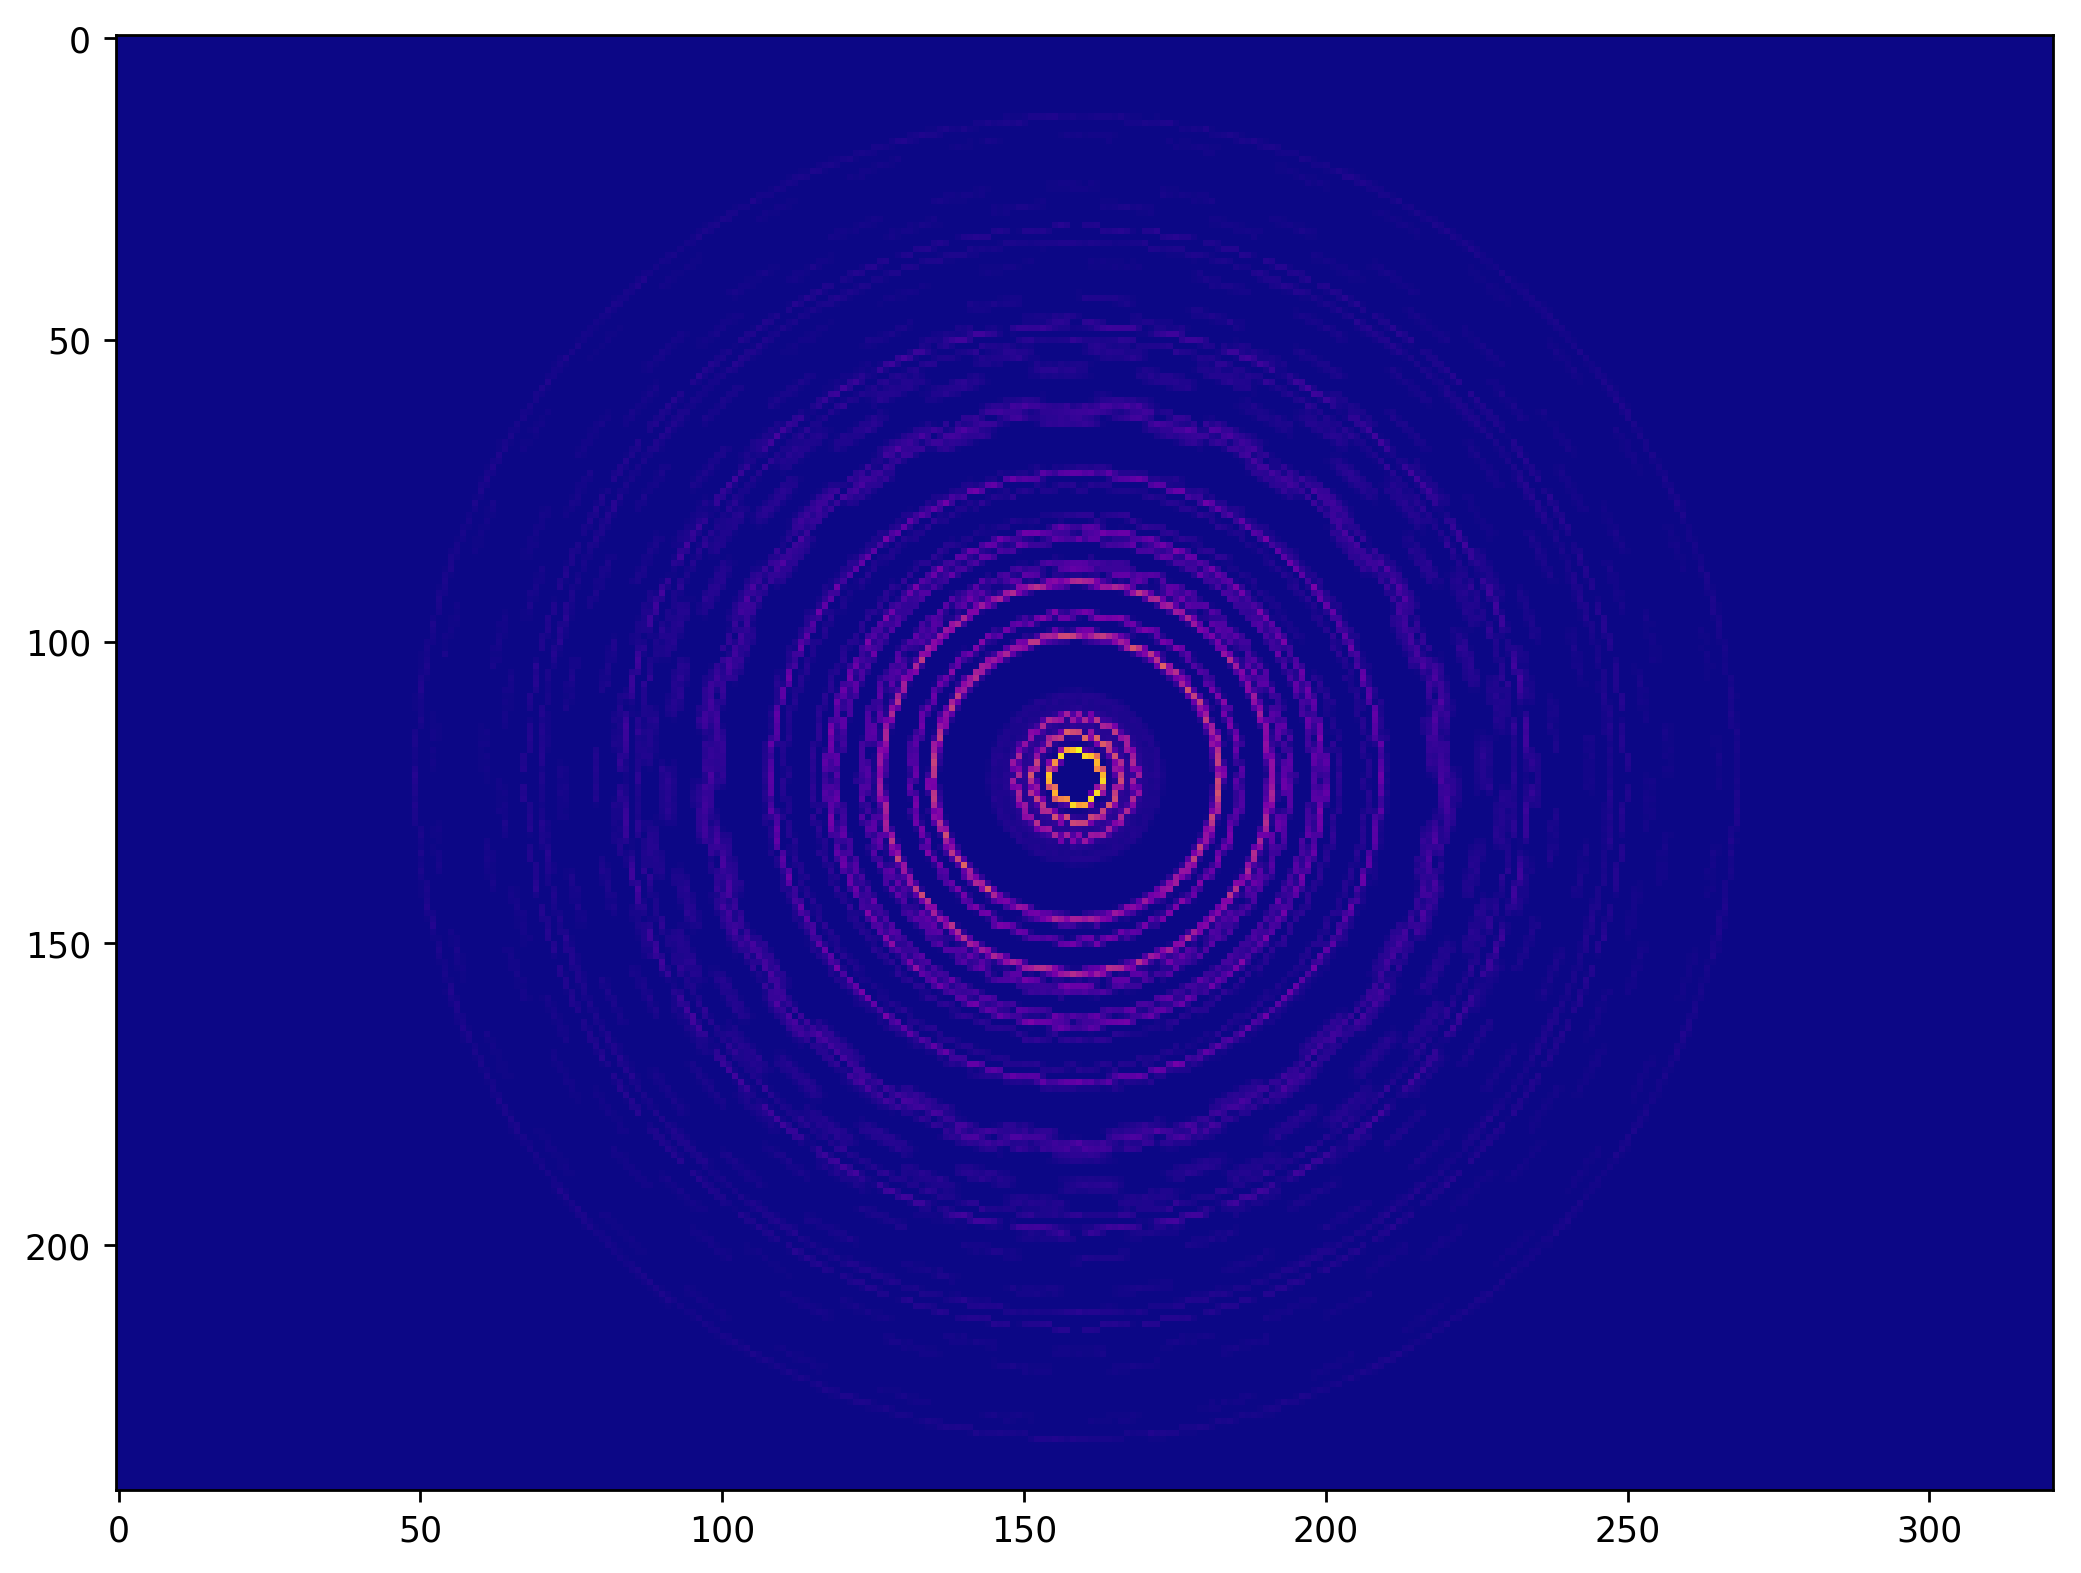
\includegraphics[width=\linewidth]{resources/images/experiment_cms_tracking_2}
    \caption{Subfigure 2}
    \label{fig:experiment_cms_input_2}
  \end{subfigure}
  \caption{Pixel-binned data representation of the hits which occurred in two different collisions.}
  \label{fig:experiment_cms_tracking}
\end{figure}

\subsection{Model Development}
\label{sec:experiment_cms_model_development}
